\section{Tree-Based Ensemble Learners} \label{sec:tree}
In this section, we explored the tree-based ensemble learners. 
\subsection{Random Forests} \label{sub: rf}
The essential idea in bagging is to average many noisy but approximately unbiased models, since trees is of instability due to its the hierarchical nature. However, if each tree generated in bagging is identically distributed but not necessarily independent, the correlation of the pairs of bagged trees would limit the benefits of averaging. Random Forest decorrelate the trees via split-variable randomization. Besides, Random Forest does not increase the variance too much, which is achieved through the random selection of split predictors \cite{Friedman:2001:ESL}.\\ 
For \textbf{GradCafe} dataset, natural splines of the numeric predictors significantly improve the performance of Random Forests, according to the metric, AUC. 
\begin{table}[h]
    \centering
    \begin{tabular}{|c|c|c|}
      \hline 
    Parameter & Value & Explanation \\ 
    \hline 
        \var{mtry} & 9 & Randomly Selected Predictors\\
    \hline 
        \var{splitrule} & extratrees & Splitting Rule \\
        \hline 
        \var{min.node.size} & 6 & Minimum size of terminal nodes \\
    \hline 
    \end{tabular}
    \caption{The value of tuning parameters used in Random Forests.}
    \label{tab:rf}
\end{table}
By 5-fold cross validation with the metric AUC, the value of tuning parameters are chosen as shown in the Table \ref{tab:rf}. \\
Figure \ref{fig: xgb} displays the variable importance for each of the predictor variables. \var{uni\_pub}, \var{decision\_month}, and \var{uni\_faculty} are predominantly relevant with the result of application. \var{GRE} and \var{GPA} have roughly half relevance of \var{uni\_pub}, whereas others do not show strong relevance. The AUC of training set is 0.8361. 
\begin{figure}[htb]
    \centering
    \begin{subfigure}{.5\linewidth}
	\centering
	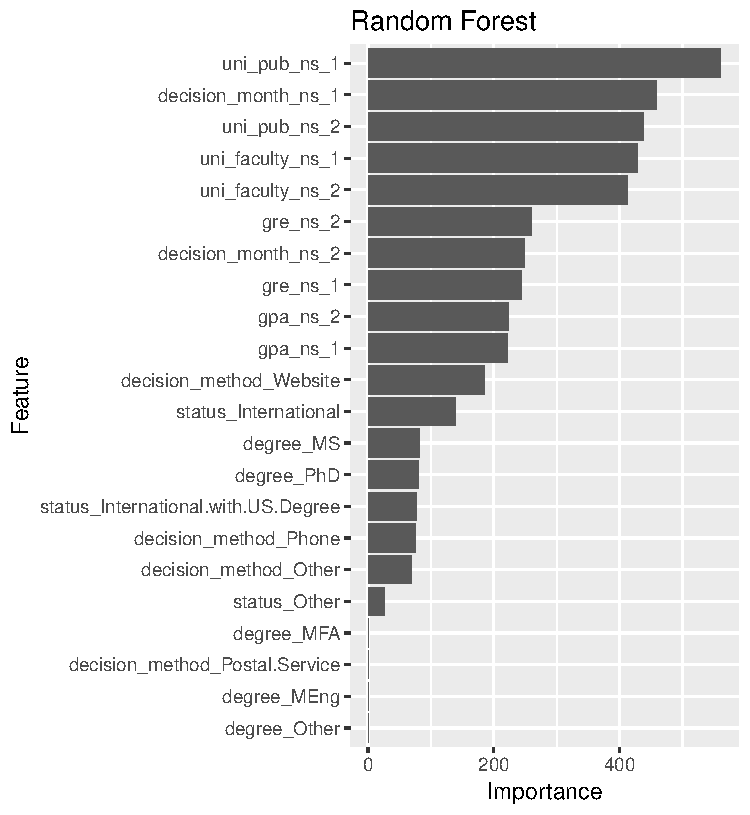
\includegraphics[width = \linewidth]{RF.pdf}
	\caption{Variable importace plots for the classification random forest grown on the \textbf{GradCafe} data.}
	\label{fig:rf}
    \end{subfigure}%
    \begin{subfigure}{.5\linewidth}
    \centering
    \includegraphics[width = \linewidth]{xgboost.pdf}
    \caption{The predictor variable importance in descending order for \textbf{GradCafe} dataset using XGBoost.}
    \label{fig: xgb}
\end{subfigure}
    \caption{Feature selection for \noun{GradCafe} ensemble learner.}
\end{figure}
The AUC of random forest on test data is 0.7558307. 

\subsection{eXtreame Gradient Boosting} \label{sub: xgb}
XGBoost is a scalable end-to-end tree boosting system, which uses far fewer resources than existing systems in billions of examples. The key problem in tree learning is to find the best split, and XGBoost uses the exact greedy algorithm. The novel tree learning algorithm of XGBoost algorithm is proposed for handling sparse data, and a theoretically justified weighted quantile sketch for approximate tree learning proposes candidate split points. The sparsity-aware split finding speeds up the computation time. Besides, the tuning parameter $Column Subsampling$ is borrowed from Random Forest. \\
Time complexity $O(Kd\left\|\mathbf{x}\right\|_0+\left\|\mathbf{x}\right\|_0\log B)$, where $d$ is the maximum depth of the tree, $K$ is the total number of trees, $B$ is the maximum number of rows in each block and $\left\|\mathbf{x}\right\|_0$ denotes the number of non-missing entries in the training data \cite{chen:2016:xgboost}. \\
The design matrix is made by using R library, {\itshape recipe} in the similar as mentioned before. R library, {\itshape xgboost}, is used for fitting XGBoost. \\
After evaluating the variable importance, we selected following interaction terms, including interactions between $status$ and $uni\_pub$, $gpa$ and $gre$, as well as $gre$ and $degree$. 
By 5-fold cross validation with the metric AUC, the tuning parameters are chosen as shown in the Table \ref{tab:xgbpar}
\begin{table}[h]
    \centering
    \begin{tabular}{|c|c|c|}
   \hline 
    Parameter & Value & Explanation \\ 
        \hline
        \var{eta} & 0.005 & Shrinkage\\
        \hline 
        \var{max\_depth} & 9 & Max Tree Depth \\
        \hline 
        \var{subsample} & 0.6 & Subsample Percentage\\
        \hline 
        \var{Colsample\_bytree} & 0.9 & Subsample Ratio of Columns \\
        \hline 
    \end{tabular}
    \caption{The value of tuning parameters used in XGBoost.}
    \label{tab:xgbpar}
\end{table}
Figure \ref{fig: xgb} displays the variable importance for each of the predictor variables. Similar to random forests, \var{publications} and \var{faculty} are the two most relevant predictors. \var{decision\_month} has the third high relevance with them, which is consistent with GLM and GAM. The interaction between \var{GPA} and \var{GRE} has roughly half the relevance of \var{decision\_month}, even  higher relevance of \var{GPA} and \var{GRE}, wheras the others are somewhat less influential.  \\

One important purpose of model fitting is to classify new data. The model performance with the binomial response in \textbf{GradCafe} is measured by AUC. The AUC of XGBoost prediction is 0.8542 on the test data. \\
